\documentclass[sigconf]{acmart}

\usepackage{hyperref}

%\usepackage{endfloat}
%\renewcommand{\efloatseparator}{\mbox{}} % no new page between figures

\usepackage{booktabs} % For formal tables

\settopmatter{printacmref=false} % Removes citation information below abstract
\renewcommand\footnotetextcopyrightpermission[1]{} % removes footnote with conference information in first column
\pagestyle{plain} % removes running headers




\begin{document}
	\title {A comparative study of Kubernetes and Docker Swarm and Advantages of Singularity Container to HPC World}
	
	
	\author{Anand Sriramulu}
	\orcid{1234-5678-9012}
	\affiliation{%
		\institution{Indiana University}
		\streetaddress{107 S Indiana Ave}
		\city{Bloomington} 
		\state{Indiana}
		\country{USA}
		\postcode{47405}
	}
	\email{asriram@iu.edu}
	
	
	% The default list of authors is too long for headers}
	\renewcommand{\shortauthors}{Anand S}
	
	
	\begin{abstract}
		Comparing Kubernetes and Docker Swarm Orchestrations, Discuss on the advantages of the Singularity Containers over the others
	\end{abstract}
	
	\keywords{i523, hid338, Data Science, Docker, Containers, Big Data Analytics, Cloud Computing, Docker Swarm, Kubernetes, Singularity}
	
	\maketitle
	
	\section{Introduction}
	Technology professional see the advantage of using a microservices architecture, wherein the application comprises of loosely coupled
	components, such as load balancers, caching proxies, message brokers, web servers, application services, and databases.
	The use of microservices allows developers to quickly create applications. In addition, this architecture saves a tremendous
	amount of resources in scaling applications, since each component can be scaled separately.
	Containers make it easy to deploy and run applications using the microservices architecture. They are lighter-weight compared
	to VMs and make more efficient use of the underlying infrastructure. Containers are meant to make it easy to scale applications,
	meet fluctuating demands, and move apps seamlessly between different environments or clouds. 
	Container orchestration tools can provide placement, scheduling, deployment, updates, health monitoring, scaling and failover functionality. 
	\cite{Container-Orchestration}	
	\section{Container Orchestration Functionalities }
	Here are some of the capabilities that a modern container orchestration platform will typically provide:
	\subsection{Provisioning}
	Container orchestration tools can provision or schedule containers within the cluster and launch them. These tools can
	determine the right placement for the containers by selecting an appropriate host based on the specified constraints such
	as resource requirements, location afinity etc. The underlying goal is to increase utilization of the available resources.
	Most tools will be agnostic to the underlying infrastructure provider and, in theory, should be able to move containers
	across environments and clouds. \cite{Provisioning}
	\subsection{Configuration-as-text}
	Container orchestration tools can load the application blueprint from a schema defined in YAML or JSON. Defining the
	blueprint in this manner makes it easy for DevOps teams to edit, share and version the configurations and provide repeatable
	deployments across development, testing and production.  \cite{Configuration-as-text}
	\subsection{Monitoring}
	Container orchestration tools will track and monitor the health of the containers and hosts in the cluster. If a container
	crashes, a new one can be spun up quickly. If a host fails, the tool will restart the failed containers on another host. It will also
	run specified health checks at the appropriate frequency and update the list of available nodes based on the results. In short,
	the tool will ensure that the current state of the cluster matches the configuration specified. 

	\subsection{Service Discovery}
	Since containers encourage a microservices based architecture, service discovery becomes a critical function and is provided
	in different ways by container orchestration platforms e.g. DNS or proxy-based etc. For example, a web application front-end
	dynamically discovering another microservice or a database. 
	\subsection{Rolling Upgrades and Rollback }
	Some orchestration tools can perform 'rolling upgrades' of the application where a new version is applied incrementally
	across the cluster. Traffic is routed appropriately as containers go down temporarily to receive the update. A rolling update
	guarantees a minimum number of "ready" containers at any point, so that all old containers are not replaced if there aren't
	enough healthy new containers to replace them. If, however, the new version doesn't perform as expected then the
	orchestration tool may also be able to rollback the applied change. 
	\subsection{Policies for Placement, Scalability etc.}	
	Container orchestration tools provide a way to define policies for host placement, security, performance and high availability.
	When configured correctly, container orchestration platforms can enable organizations to deploy and operate containerized
	application workloads in a secure, reliable and scalable way. For example, an application can be scaled up automatically based
	on CPU usage of the containers. 
	\subsection{Administration}	
	Container orchestration tools should provide mechanisms for administrators to deploy, configure and setup. An extensible
	architecture will connect to external systems such as local or cloud storage, networking systems etc. They should connect to
	existing IT tools for SSO, RBAC etc. 
	
	\section{Kubernetes}
	Kubernetes is a Goolge product and they used it for their running their heavy workloads in production.	
	Kubernetes website says, "Kubernetes is an open-source system for automating deployment, scaling, and management of containerized applications."
	\cite{Kubernetes}
\begin{figure}
	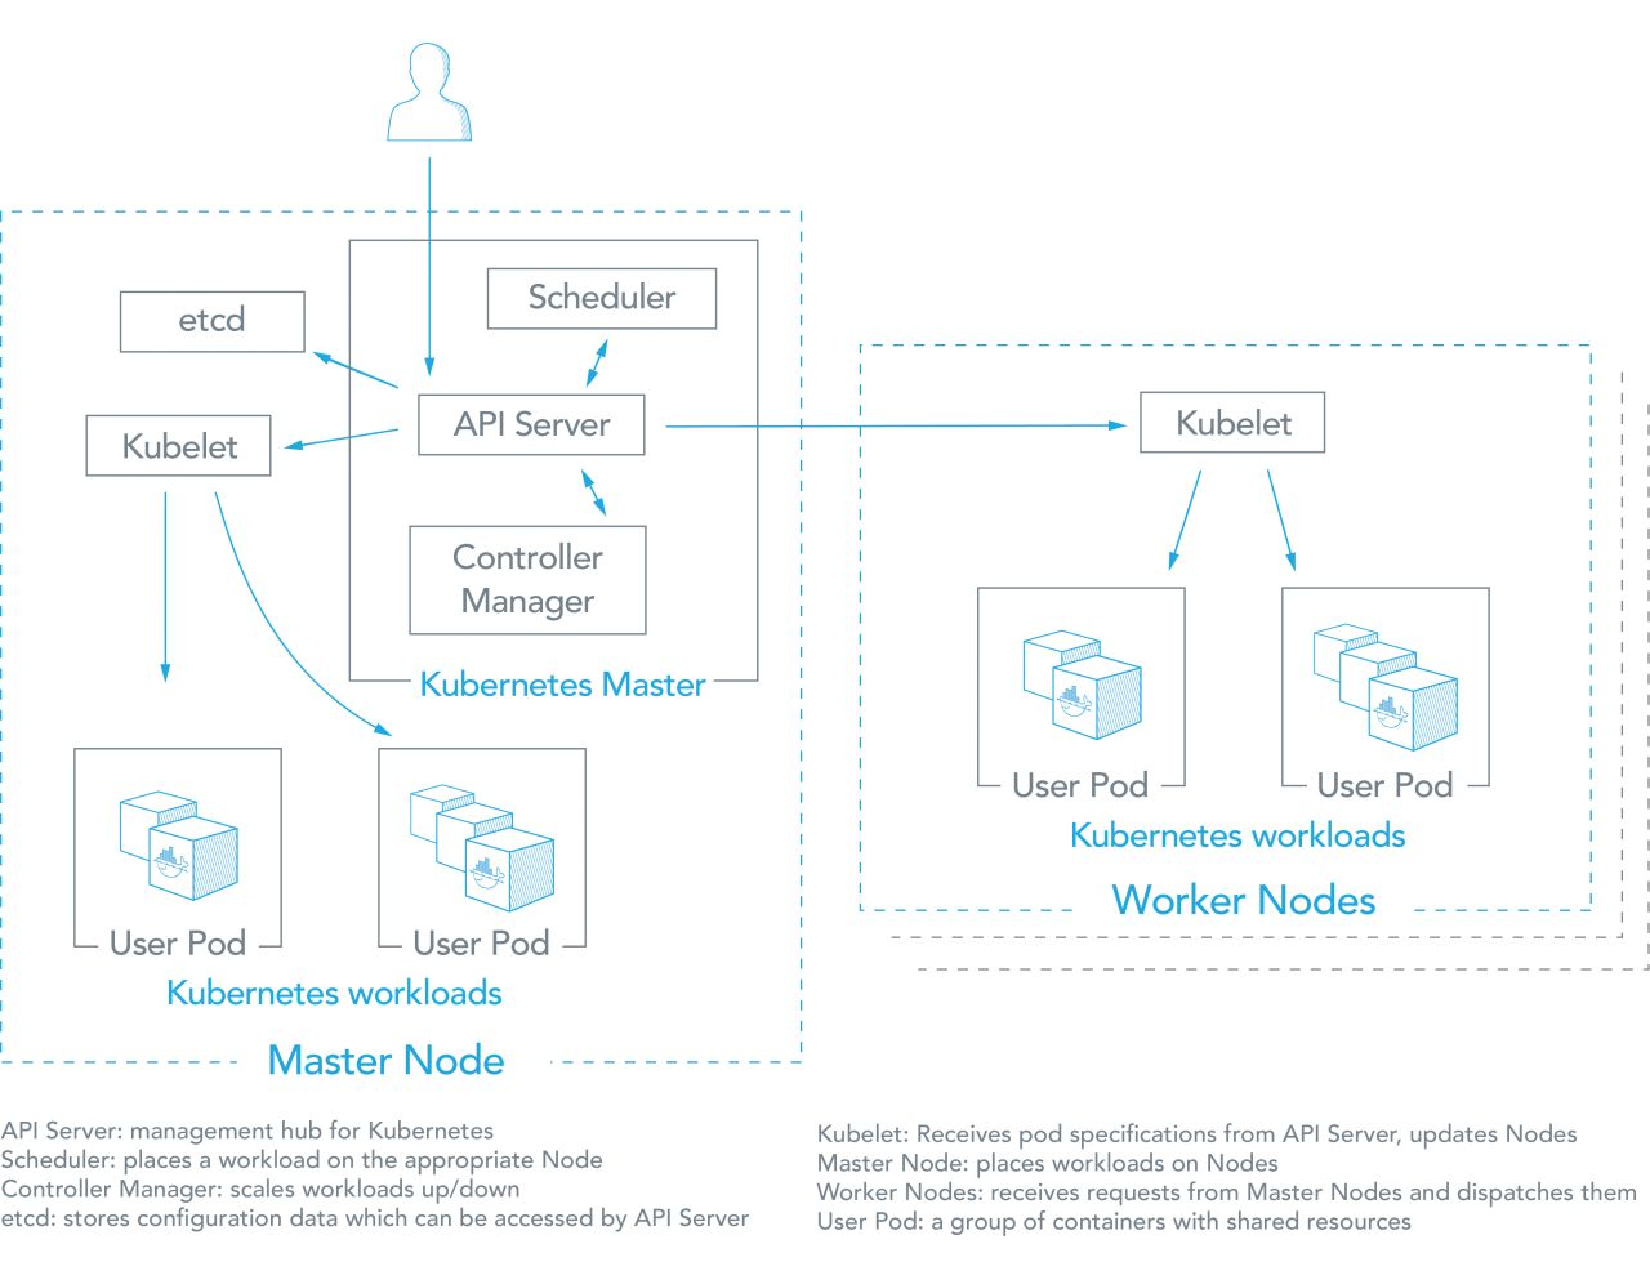
\includegraphics[width=0.5\textwidth]{images/Kubernetes}
	\caption{Kubernetes Nodes Illustration \cite{Platform9}.} \label{fig:figure1} 
\end{figure}

	\section{Docker Swarm}
	Docker swarm is a simple container orchestrion and yet it's powerful. It's embedded part of the docker engine and provides cluster management 
	and orchestration features.
\begin{figure}
	\includegraphics[width=0.5\textwidth]{images/DockerSwarm}
	\caption{Docker Swarm Architecture \cite{Platform9}.} \label{fig:figure2} 
\end{figure}

\section{Kubernetes vs Docker Swarm}
Both the contrainer orchestration offers similar functionalities, but I will discuss on the pros and cons here.
\cite{kubernetes-vs-docker-swarm}
\subsection{Application definition}
Kubernetes can be deployed in combination of pods and micro-services. Docker, whereas applications can be deployed as micro-services.
\subsection{Installation and Setup}

Kubernetes is not very easy in terms of setup, but Google provides good documentation for the setup. It takes lot of time for the developer to get the setup done.
On the other hand, Docker Swarm doesn't need much learning for the developers or devops and has easy process to setup and manage with the help of Command Line Interface (CLI).
Overall, Docker wins here.

\subsection{Monitoring and Logging}
Both Kubernetes and Docker Swarm doesnt provide inbuilt support but extent offers logging and monitoring thru third party libraries. 
With Docker, DataDog, Reimann, Retrace and Sumo Logic can be used.
With Kubernetes, Kibana and ElasticSearch can be used for Logging and Influx, Grafana, Heapster for Monitoring.

\subsection{Size and Performance}
Both can support 1000 node clusters in which each cluster can support up to 30,000 containers.

\section {Singularity Container and Features}
As per Singularity website "Singularity containers can be used to package entire scientific workflows, software and libraries, and even data. This means that you don't have to ask your cluster admin to install anything for you - you can put it in a Singularity container and run"

Singularity containers is different from other containers due to the following aspects
Application Portability - Single Image File which contain all dependencies. Reproducibility, run cross platform and support legacy operating system and applications.
Docker Integration - It can convert Docker images into Singularity images easily
User Group Focus - It focuses on Scientific Application Users
Security Model - It's the key aspect that it can be used with unprivileged permissions and doesn't require a separate daemon process. In which it highly useful in HPC workloads
\cite{}
\bibliographystyle{ACM-Reference-Format}
\bibliography{report} 

\end{document}
